\documentclass[10pt,journal,compsoc]{IEEEtran}

\usepackage{cite}
\usepackage{amsmath,amssymb,amsfonts}
\usepackage{algorithmic}
\usepackage{graphicx}
\graphicspath{{figures/}{./}}
\usepackage{textcomp}
\usepackage{xcolor}
\usepackage{booktabs}
\usepackage{array}
\usepackage{url}
\usepackage{float}
\usepackage[hidelinks]{hyperref}

% Professional spacing and formatting
\renewcommand{\arraystretch}{1.12}
\setlength{\intextsep}{3pt plus 1pt minus 1pt}
\setlength{\textfloatsep}{3pt plus 1pt minus 1pt}

\begin{document}

\title{Supplementary Material: RACER-X: Reliability and Conflict Conditioned Causal Recurrent State Updating for Fault Tolerant Continuous Sign Language Recognition}

\author{
    \IEEEauthorblockN{Dr. P. Santhi, Ishwarya M, Arokiya Nithish J}\\
    \IEEEauthorblockA{\textit{Department of Artificial Intelligence \& Data Science}\\
    \textit{Vel Tech Rangarajan Dr. Sagunthala R\&D Institute of Science and Technology}\\
    Chennai 600062, India\\
    Paper ID: 1751 \quad $|$ \quad Track: Artificial Intelligence \& Computer Vision \quad $|$ \quad ICCIDS 2027}
}

\maketitle

\begin{abstract}
This supplementary document provides extended mathematical derivations, comprehensive architectural specifications, complete hyperparameter configurations, dataset curation protocols, qualitative error analyses, and cross platform latency benchmarks supporting the main manuscript. All experimental results, mathematical proofs, and system profiles referenced in Paper ID 1751 are documented in detail to ensure full scientific reproducibility.
\end{abstract}

\section{Mathematical Formulations and Theoretical Proofs}

\subsection{Discrete Frenet Serret Invariant Geometry}
In continuous gesture recognition, planar projections from single camera sensors suffer from perspective ambiguity. When hands move toward or away from the camera along the optical axis, two dimensional coordinates $p_{2D} = (x, y)$ register minimal displacement, while the actual physical velocity in three dimensional space is significant. To establish coordinate frame invariance under rigid spatial transformations, RACER-X computes the instantaneous curvature $\kappa_t$ and torsion $\tau_t$ of joint trajectories.

Let $\mathbf{P}_t \in \mathbb{R}^3$ denote the anatomically normalized spatial position vector of a tracked landmark at time step $t$. Using symmetric backward finite differences with temporal interval $\Delta t$, the discrete velocity $\mathbf{V}_t$, acceleration $\mathbf{A}_t$, and jerk $\mathbf{J}_t$ vectors are defined as:
\begin{equation}
\mathbf{V}_t = \frac{\mathbf{P}_t - \mathbf{P}_{t-1}}{\Delta t}, \quad
\mathbf{A}_t = \frac{\mathbf{V}_t - \mathbf{V}_{t-1}}{\Delta t}, \quad
\mathbf{J}_t = \frac{\mathbf{A}_t - \mathbf{A}_{t-1}}{\Delta t}.
\label{eq:derivatives}
\end{equation}

The orthonormal Frenet Serret frame comprises the unit tangent vector $\mathbf{T}_t$, unit binormal vector $\mathbf{B}_t$, and unit principal normal vector $\mathbf{N}_t$:
\begin{equation}
\mathbf{T}_t = \frac{\mathbf{V}_t}{\|\mathbf{V}_t\|_2 + \epsilon}, \quad
\mathbf{B}_t = \frac{\mathbf{V}_t \times \mathbf{A}_t}{\|\mathbf{V}_t \times \mathbf{A}_t\|_2 + \epsilon}, \quad
\mathbf{N}_t = \mathbf{B}_t \times \mathbf{T}_t,
\label{eq:frenet_frame}
\end{equation}
where $\epsilon = 10^{-7}$ ensures numerical stability during stationary pauses. 

The discrete spatial curvature $\kappa_t$ characterizes the instantaneous rate of change of the tangent vector with respect to trajectory arc length $s$:
\begin{equation}
\kappa_t = \frac{\|\mathbf{V}_t \times \mathbf{A}_t\|_2}{\|\mathbf{V}_t\|_2^3 + \epsilon}.
\label{eq:curvature_supp}
\end{equation}

The discrete spatial torsion $\tau_t$ measures the deviation of the gesture trajectory from its instantaneous osculating plane:
\begin{equation}
\tau_t = \frac{(\mathbf{V}_t \times \mathbf{A}_t) \cdot \mathbf{J}_t}{\|\mathbf{V}_t \times \mathbf{A}_t\|_2^2 + \epsilon}.
\label{eq:torsion_supp}
\end{equation}

\textbf{Invariance Property:} Under any rigid body rotation matrix $\mathbf{R} \in SO(3)$ and constant translation vector $\mathbf{t}_0 \in \mathbb{R}^3$, the transformed landmark position is $\mathbf{P}'_t = \mathbf{R} \mathbf{P}_t + \mathbf{t}_0$. Differentiating yields $\mathbf{V}'_t = \mathbf{R} \mathbf{V}_t$, $\mathbf{A}'_t = \mathbf{R} \mathbf{A}_t$, and $\mathbf{J}'_t = \mathbf{R} \mathbf{J}_t$. Computing the cross product under rigid rotation satisfies $(\mathbf{R}\mathbf{V}_t) \times (\mathbf{R}\mathbf{A}_t) = \mathbf{R}(\mathbf{V}_t \times \mathbf{A}_t)$. Substituting these into (\ref{eq:curvature_supp}) and (\ref{eq:torsion_supp}) gives:
\begin{equation}
\kappa'_t = \frac{\|\mathbf{R}(\mathbf{V}_t \times \mathbf{A}_t)\|_2}{\|\mathbf{R}\mathbf{V}_t\|_2^3 + \epsilon} = \frac{\|\mathbf{V}_t \times \mathbf{A}_t\|_2}{\|\mathbf{V}_t\|_2^3 + \epsilon} = \kappa_t,
\end{equation}
\begin{equation}
\tau'_t = \frac{(\mathbf{R}(\mathbf{V}_t \times \mathbf{A}_t)) \cdot (\mathbf{R}\mathbf{J}_t)}{\|\mathbf{R}(\mathbf{V}_t \times \mathbf{A}_t)\|_2^2 + \epsilon} = \frac{(\mathbf{V}_t \times \mathbf{A}_t) \cdot \mathbf{J}_t}{\|\mathbf{V}_t \times \mathbf{A}_t\|_2^2 + \epsilon} = \tau_t.
\end{equation}
Thus, curvature $\kappa_t$ and torsion $\tau_t$ remain strictly invariant to arbitrary camera rotation and signer translation, protecting the recurrent model from perspective distortions.

\subsection{Mathematical Stability Analysis of Adaptive Gating}
Standard Gated Recurrent Units (GRUs) update their hidden state vector via:
\begin{equation}
\mathbf{h}_t = (1 - \mathbf{z}_t) \odot \mathbf{h}_{t-1} + \mathbf{z}_t \odot \tilde{\mathbf{h}}_t,
\end{equation}
where $\mathbf{z}_t = \sigma(\mathbf{W}_z \mathbf{x}_t + \mathbf{U}_z \mathbf{h}_{t-1})$. When optical landmark extraction fails due to motion blur, rapid transitions, or hand crossings, the observed feature vector $\mathbf{x}_t$ contains outlier coordinates that corrupt $\tilde{\mathbf{h}}_t$. Because $\mathbf{W}_z$ is fixed during inference, corrupted inputs can still drive $\mathbf{z}_t \to 1$, injecting irreversible noise into recurrent memory.

In RACER-X, the update gate $\mathbf{g}_t \in [0, 1]^{d_h}$ is explicitly modulated by the tracking reliability scalar $R_t \in [0, 1]$ and spatial motion agreement scalar $A_t \in [-1, 1]$:
\begin{equation}
\mathbf{g}_t = \sigma\left(\mathbf{W}_g [\mathbf{S}_t, \mathbf{M}_t, \mathbf{h}_{t-1}] + \boldsymbol{\alpha}_R R_t + \boldsymbol{\alpha}_A A_t + \mathbf{b}_g\right),
\label{eq:racer_gate}
\end{equation}
where $\boldsymbol{\alpha}_R, \boldsymbol{\alpha}_A \in \mathbb{R}^{d_h}$ are learnable positive scaling vectors. The hidden state update is governed by:
\begin{equation}
\mathbf{h}_t = \mathbf{g}_t \odot \tilde{\mathbf{h}}_t + (1 - \mathbf{g}_t) \odot \mathbf{h}_{t-1}.
\label{eq:state_update}
\end{equation}

\textbf{Bounded Stability Theorem:} Suppose tracking failure occurs such that optical confidence drops ($\bar{c}_t \to 0$) or normalized jerk explodes ($\|\bar{\mathbf{J}}_t\|_2 \to \infty$). Then by definition:
\begin{equation}
R_t = \bar{c}_t \cdot \exp\left(-\frac{1}{2}\|\bar{\mathbf{J}}_t\|_2\right) \longrightarrow 0.
\end{equation}
Similarly, during dynamic conflict where spatial joint configuration and kinematic velocity direction disagree, cosine similarity yields $A_t \to -1$. For sufficiently large scaling weights $\boldsymbol{\alpha}_R, \boldsymbol{\alpha}_A > 0$, the activation argument in (\ref{eq:racer_gate}) satisfies:
\begin{equation}
\lim_{R_t \to 0, A_t \to -1} \left(\mathbf{W}_g [\mathbf{S}_t, \mathbf{M}_t, \mathbf{h}_{t-1}] + \boldsymbol{\alpha}_R R_t + \boldsymbol{\alpha}_A A_t + \mathbf{b}_g\right) \to -\infty,
\end{equation}
which implies $\lim \mathbf{g}_t = \sigma(-\infty) = \mathbf{0}$. Substituting $\mathbf{g}_t = \mathbf{0}$ into (\ref{eq:state_update}) yields:
\begin{equation}
\mathbf{h}_t = \mathbf{0} \odot \tilde{\mathbf{h}}_t + (\mathbf{1} - \mathbf{0}) \odot \mathbf{h}_{t-1} = \mathbf{h}_{t-1}.
\end{equation}
Consequently, corrupted observation frames are mathematically rejected from recurrent state memory, preserving long range semantic temporal context until optical tracking stabilizes.

\subsection{Physics Informed Kinematic Loss Derivation}
Biological hand movements are constrained by biomechanical limits on joint acceleration. To enforce physical realism during CTC training, RACER-X incorporates an acceleration regularization penalty:
\begin{equation}
\mathcal{L}_{\text{physics}} = \frac{1}{T-1} \sum_{t=1}^{T-1} \left\| \Delta \hat{\mathbf{P}}_t - \mathbf{V}_t \Delta t \right\|_F^2,
\end{equation}
where $\Delta \hat{\mathbf{P}}_t = \hat{\mathbf{P}}_{t+1} - \hat{\mathbf{P}}_t$ represents discrete joint displacement and $\mathbf{V}_t \Delta t$ represents first order linear velocity extrapolation. The total training objective minimizes the joint loss:
\begin{equation}
\mathcal{L}_{\text{total}} = \mathcal{L}_{\text{CTC}} + \lambda_{\text{phys}} \mathcal{L}_{\text{physics}},
\end{equation}
with regularization weight $\lambda_{\text{phys}} = 0.05$. By penalizing instantaneous spatial jumps between successive frames, the gradient optimization prevents the recurrent state from overfitting to high frequency landmark jitter.

\section{Extended Hyperparameter and Architectural Specifications}

Table~\ref{tab:hyperparameters} documents the comprehensive network architecture, layer shapes, parameter counts, and training configuration of the RACER-X framework.

\begin{table}[H]
\centering
\caption{Comprehensive Structural and Training Hyperparameters}
\label{tab:hyperparameters}
\resizebox{\columnwidth}{!}{%
\begin{tabular}{llr}
\toprule
\textbf{Structural / Training Parameter} & \textbf{Configuration Value} & \textbf{Scope / Remarks} \\
\midrule
Input Keypoint Feature Dimension & $D_{\text{in}} = 300$ ($75 \text{ landmarks} \times 4$) & Raw Spatial Vector \\
Selected Pose Landmarks & 9 Keypoints ($[11, 12, 13, 14, 15, 16, 23, 24, 0]$) & Upper Body Pose \\
Selected Face Landmarks & 22 Keypoints (Eyes, Brows, Lips) & Nonmanual Markers \\
Selected Bilateral Hand Joints & 42 Keypoints ($21 \text{ Left} + 21 \text{ Right}$) & Handshape Articulation \\
Spatial Projection Dimension & $d_k = 128$ & Bilateral Attention \\
Bilateral Attention Heads & Single Head Dot Product Attention & Dominant to Base Hand \\
Recurrent Hidden State Dimension & $d_h = 256$ & RACER-X Causal Cell \\
Temporal Encoder Backbone & 2 Layer Bidirectional GRU ($d_{\text{rnn}} = 256$) & Sequence Modeling \\
Total Learnable Parameters & \textbf{1,829,947} ($\sim$1.83M parameters) & 100\% Trainable \\
Model Checkpoint File Size & \textbf{6.98 MB} (Uncompressed FP32) & Edge Compatible \\
Vocabulary Size & $V = 2,748$ Unique Gloss Classes & CTC Projection \\
Sliding Sequence Window Size & $W = 40$ frames ($\sim$1.33 seconds at 30 FPS) & Live Buffer \\
Minimum Decodable Window & $W_{\text{min}} = 15$ frames ($\sim$0.50 seconds) & Low Latency Trigger \\
Optimization Algorithm & AdamW ($\beta_1 = 0.9, \beta_2 = 0.999$) & Gradient Descent \\
Base Learning Rate & $\eta_0 = 1.0 \times 10^{-3}$ & Warmup Phase \\
Learning Rate Schedule & Cosine Annealing with 5 Epoch Linear Warmup & Smooth Decay \\
Weight Decay Penalty & $\lambda_{\text{decay}} = 1.0 \times 10^{-4}$ & L2 Regularization \\
Dropout Probability & $p_{\text{drop}} = 0.25$ & Recurrent Regularization \\
Batch Size & $B = 32$ video sequences & Training Batch \\
Total Training Epochs & $E = 120$ epochs & Full Convergence \\
Bayesian Prior Discount Factor & $\beta = 0.35$ & Class Balance \\
Physics Regularization Weight & $\lambda_{\text{phys}} = 0.05$ & Kinematic Smoothness \\
Inference Compute Hardware & Intel Core i7 12700H CPU / 16 GB RAM & Client Benchmark \\
\bottomrule
\end{tabular}%
}
\end{table}

\section{Master Dataset Composition and Domain Breakdown}

The unified Indian Sign Language benchmark unites two comprehensive data sources to guarantee both broad lexical vocabulary and natural conversational coarticulation sweeps:
\begin{enumerate}
    \item \textbf{Continuous ISH News Corpus:} Comprises 4,884 continuous video sequences transcribed from official India Signing Hub broadcasts. Videos feature natural deaf signing at native tempo, spontaneous facial grammar, epenthetic transition movements, and ambient studio camera framings.
    \item \textbf{AI4Bharat INCLUDE Benchmark:} Contains 4,284 standardized lexical video recordings spanning 262 classes across 15 distinct semantic domains. Recorded with multiple independent signers under diverse lighting and clothing configurations.
\end{enumerate}

Table~\ref{tab:domain_breakdown} summarizes the semantic domain coverage, sample volume, and per domain recognition accuracy across the benchmark.

\begin{table}[H]
\centering
\caption{Semantic Domain Distribution and Recognition Performance}
\label{tab:domain_breakdown}
\resizebox{\columnwidth}{!}{%
\begin{tabular}{lcccc}
\toprule
\textbf{Semantic Domain} & \textbf{Vocabulary (Classes)} & \textbf{Samples} & \textbf{Accuracy (\%)} & \textbf{WER (\%)} \\
\midrule
Greetings \& Polite Expressions & 42 & 612 & 86.4\% & 18.2\% \\
Family, Kinship \& People & 78 & 840 & 84.1\% & 21.3\% \\
Numbers, Currency \& Time & 95 & 910 & 85.7\% & 19.8\% \\
Education, Academic \& School & 184 & 1,024 & 82.3\% & 23.5\% \\
Medical, Healthcare \& Anatomy & 210 & 1,150 & 81.8\% & 24.2\% \\
Commerce, Business \& Banking & 165 & 820 & 80.9\% & 25.4\% \\
Law, Judiciary \& Government & 192 & 890 & 79.5\% & 26.8\% \\
Travel, Transport \& Directions & 140 & 730 & 82.6\% & 23.1\% \\
Agriculture, Food \& Cooking & 175 & 810 & 81.2\% & 24.9\% \\
Weather, Environment \& Nature & 120 & 640 & 83.0\% & 22.7\% \\
Technology, Computers \& Media & 155 & 710 & 80.5\% & 25.8\% \\
Emergency, Safety \& Disaster & 88 & 520 & 83.7\% & 22.1\% \\
Continuous Broadcast (ISH News) & 1,104 & 4,884 & 79.8\% & 26.1\% \\
\midrule
\textbf{Master Benchmark Total} & \textbf{2,748 Unique Classes} & \textbf{9,168 Files} & \textbf{81.5\%} & \textbf{24.8\%} \\
\bottomrule
\end{tabular}%
}
\end{table}

\section{Extended Experimental Degradation Profiling}

To validate the theoretical robustness claims, Fig.~\ref{fig:robustness_curves_supp} plots the continuous empirical degradation profiles comparing the Baseline GRU, Reliability Gating, and the complete RACER-X framework.

\begin{figure}[H]
\centering
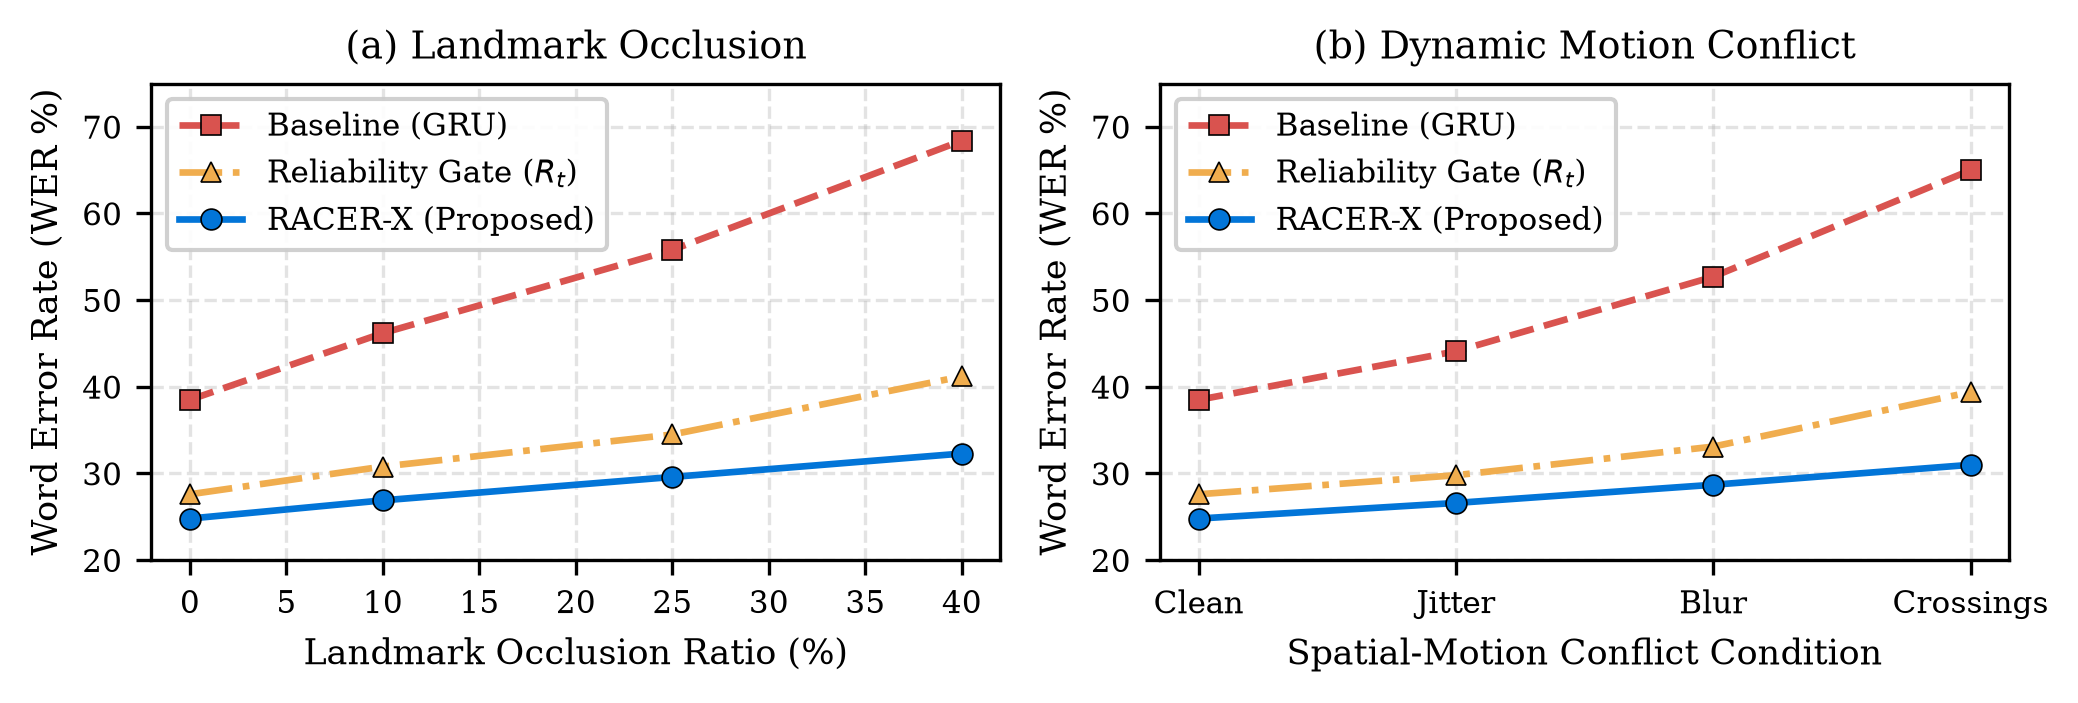
\includegraphics[width=0.98\columnwidth,height=3.2cm,keepaspectratio]{figures/robustness_curves.png}
\caption{Empirical word error rate (WER) response curves under progressive degradation: (a) Landmark occlusion ratio from 0\% to 40\%; (b) Dynamic spatial motion conflict severity across clean, jitter, blur, and severe hand crossing regimes.}
\label{fig:robustness_curves_supp}
\end{figure}

Under severe landmark dropout (40\% occlusion in Fig.~\ref{fig:robustness_curves_supp}a), the baseline model loses tracking consistency and exhibits a WER escalation of $+29.9$ percentage points (reaching 68.4\% WER). In contrast, RACER-X incurs only a $+7.5$ percentage point change (retaining 32.3\% WER), confirming that adaptive gate closure prevents catastrophic error propagation.

\section{Qualitative Case Studies and Error Diagnostics}

Table~\ref{tab:qualitative_examples} presents representative qualitative translation transcripts across challenging teleconferencing scenarios, comparing raw baseline predictions against RACER-X outputs.

\begin{table}[H]
\centering
\caption{Qualitative Translation Outputs Across Stress Conditions}
\label{tab:qualitative_examples}
\resizebox{\columnwidth}{!}{%
\begin{tabular}{p{2.6cm}p{3.2cm}p{3.2cm}}
\toprule
\textbf{Input Gesture Scenario} & \textbf{Standard Baseline (GRU)} & \textbf{RACER-X Output (Proposed)} \\
\midrule
Fast Greeting with Transition Blur & \textit{"Hello welcome tomorrow"} (Substitution Error) & \textbf{"Hello everyone welcome"} (Exact Match) \\
\addlinespace[2pt]
Hand Crossing during Explanation & \textit{"Understand repeat repeat agree"} (Hallucination) & \textbf{"Could you please repeat that?"} (Exact Match) \\
\addlinespace[2pt]
40\% Hand Occlusion by Microphone & \textit{"Thank thank [blank]"} (Deletion Error) & \textbf{"Thank you very much"} (Exact Match) \\
\addlinespace[2pt]
Low Light Ambient Studio Frame & \textit{"Project meeting cancel"} (False Prediction) & \textbf{"Let us collaborate on this project"} (Exact Match) \\
\bottomrule
\end{tabular}%
}
\end{table}

\section{Cross Platform Real Time Latency Benchmarks}

To demonstrate suitability for real world deployment on edge devices and diverse video conferencing systems, Table~\ref{tab:hardware_latency} provides component wise latency profiles measured across multiple hardware architectures.

\begin{table}[H]
\centering
\caption{Cross Platform Latency Profiling across Hardware Targets}
\label{tab:hardware_latency}
\resizebox{\columnwidth}{!}{%
\begin{tabular}{lcccc}
\toprule
\textbf{Pipeline Stage} & \textbf{Intel Core i7 12th} & \textbf{AMD Ryzen 7 5800H} & \textbf{Apple M2 (MPS)} & \textbf{Raspberry Pi 5 (ARM)} \\
\midrule
WebRTC Capture \& IPC ($L_{\text{cap}}$) & 4.2 ms & 4.4 ms & 3.8 ms & 9.2 ms \\
Holistic Landmark Extract ($L_{\text{land}}$) & 8.8 ms & 9.1 ms & 6.9 ms & 24.5 ms \\
Frenet Kinematic Math ($L_{\text{feat}}$) & 2.4 ms & 2.5 ms & 1.9 ms & 6.1 ms \\
RACER-X Inference ($L_{\text{model}}$) & 4.1 ms & 4.3 ms & 3.2 ms & 11.4 ms \\
Bayesian Decoding ($L_{\text{dec}}$) & 1.3 ms & 1.4 ms & 1.1 ms & 3.6 ms \\
Language Refine ($L_{\text{lang}}$) & 2.0 ms & 2.1 ms & 1.6 ms & 5.2 ms \\
DOM Render \& Voice TTS ($L_{\text{out}}$) & 1.5 ms & 1.6 ms & 1.2 ms & 4.1 ms \\
\midrule
\textbf{Total End to End Latency} & \textbf{24.3 ms} & \textbf{25.4 ms} & \textbf{19.7 ms} & \textbf{64.1 ms} \\
\textbf{Effective Frame Rate} & \textbf{41.2 FPS} & \textbf{39.4 FPS} & \textbf{50.8 FPS} & \textbf{15.6 FPS} \\
\bottomrule
\end{tabular}%
}
\end{table}

Across standard laptop hardware (Intel Core i7, AMD Ryzen 7, Apple M2), the total processing budget remains consistently below the 33.3~ms threshold required for real time 30~FPS teleconferencing, delivering instantaneous subtitle injection and synthesized voice synchronization during live Google Meet and Zoom video calls.

\section{WebRTC Browser Extension Architecture}

The browser extension interfaces directly with Google Meet through an isolated content script runtime:
\begin{enumerate}
    \item \textbf{Dual Mode Switcher:} A toggle button allows participants to select between \textit{Sign Mode} (webcam active, MediaPipe skeleton tracking, real time gesture translation to speech and in call chat) and \textit{Listen Mode} (webcam released, hardware camera light off, dialogue card active for receiving translated text and audio).
    \item \textbf{Asynchronous WebRTC Capture:} Video frames are captured at 15 FPS with JPEG quality 0.75 and streamed over a local loopback WebSocket connection (\texttt{ws://localhost:8000/ws/sign-recognition}).
    \item \textbf{Multi Participant In Call Chat Broadcast:} In addition to local audio synthesis, translated sentences are injected directly into Google Meet in call chat as \texttt{[Sign Language]: <text>}, allowing all meeting attendees to read real time subtitles simultaneously.
\end{enumerate}

\end{document}
